\documentclass[12pt]{scrartcl}

\usepackage[utf8]{inputenc}
\usepackage[naustrian]{babel}
\usepackage{caption}
\usepackage{graphicx}
\usepackage{verbatim}
\usepackage[T1]{fontenc}
\usepackage{lmodern}
\usepackage{subcaption}
\usepackage{amsmath}
\usepackage{mathtools}
\usepackage{amsfonts}
\usepackage{algorithm2e}
\usepackage{listings}

%pdfs
\usepackage{pdfpages}
\usepackage{tikz}

%page borders
\usepackage{geometry}
\geometry{left=2.5cm,right=2.5cm,top=3cm,bottom=2.5cm}

\usepackage{minted}
\setminted {
	%style=igor, %borland, autumn, vs
	encoding=utf-8,
	autogobble,
	tabsize=4,
	linenos,
	breaklines,
	keywordcase=upper,
	%escapeinside=||
	%bgcolor=bg
	%frame=single
}
% binary tree
\usepackage{tikz-qtree}

\newcommand{\var}{\textit}
\newcommand{\PK}[1]{\underline{\var{#1}}}
\newcommand{\FK}[1]{\textup{FK}(#1)}

\newenvironment{relationalmodel}
  {\par\medskip
   \setlength{\arraycolsep}{0pt}%
   $\begin{array}{ r l }}
   {\end{array}$
   \par\medskip}

\newenvironment{code}{\captionsetup{type=listing}}{}

%title/footer/header values
\usepackage{titling}
\title{DES3UE Übung 2}
\author{Elias Leonhardsberger}
\date{\today{}, Hagenberg}

%footer/header
%\usepackage[automark]{scrpage2}
%\pagestyle{headings}
%\clearscrheadfoot
%\ihead{\thetitle}
%\chead{\theauthor}
%\ohead{\today}
%\cfoot{Seite \pagemark}

\begin{document}
\clearpage
\thispagestyle{empty}
\begin{tikzpicture}[remember picture, overlay]
	\node at (current page.center) {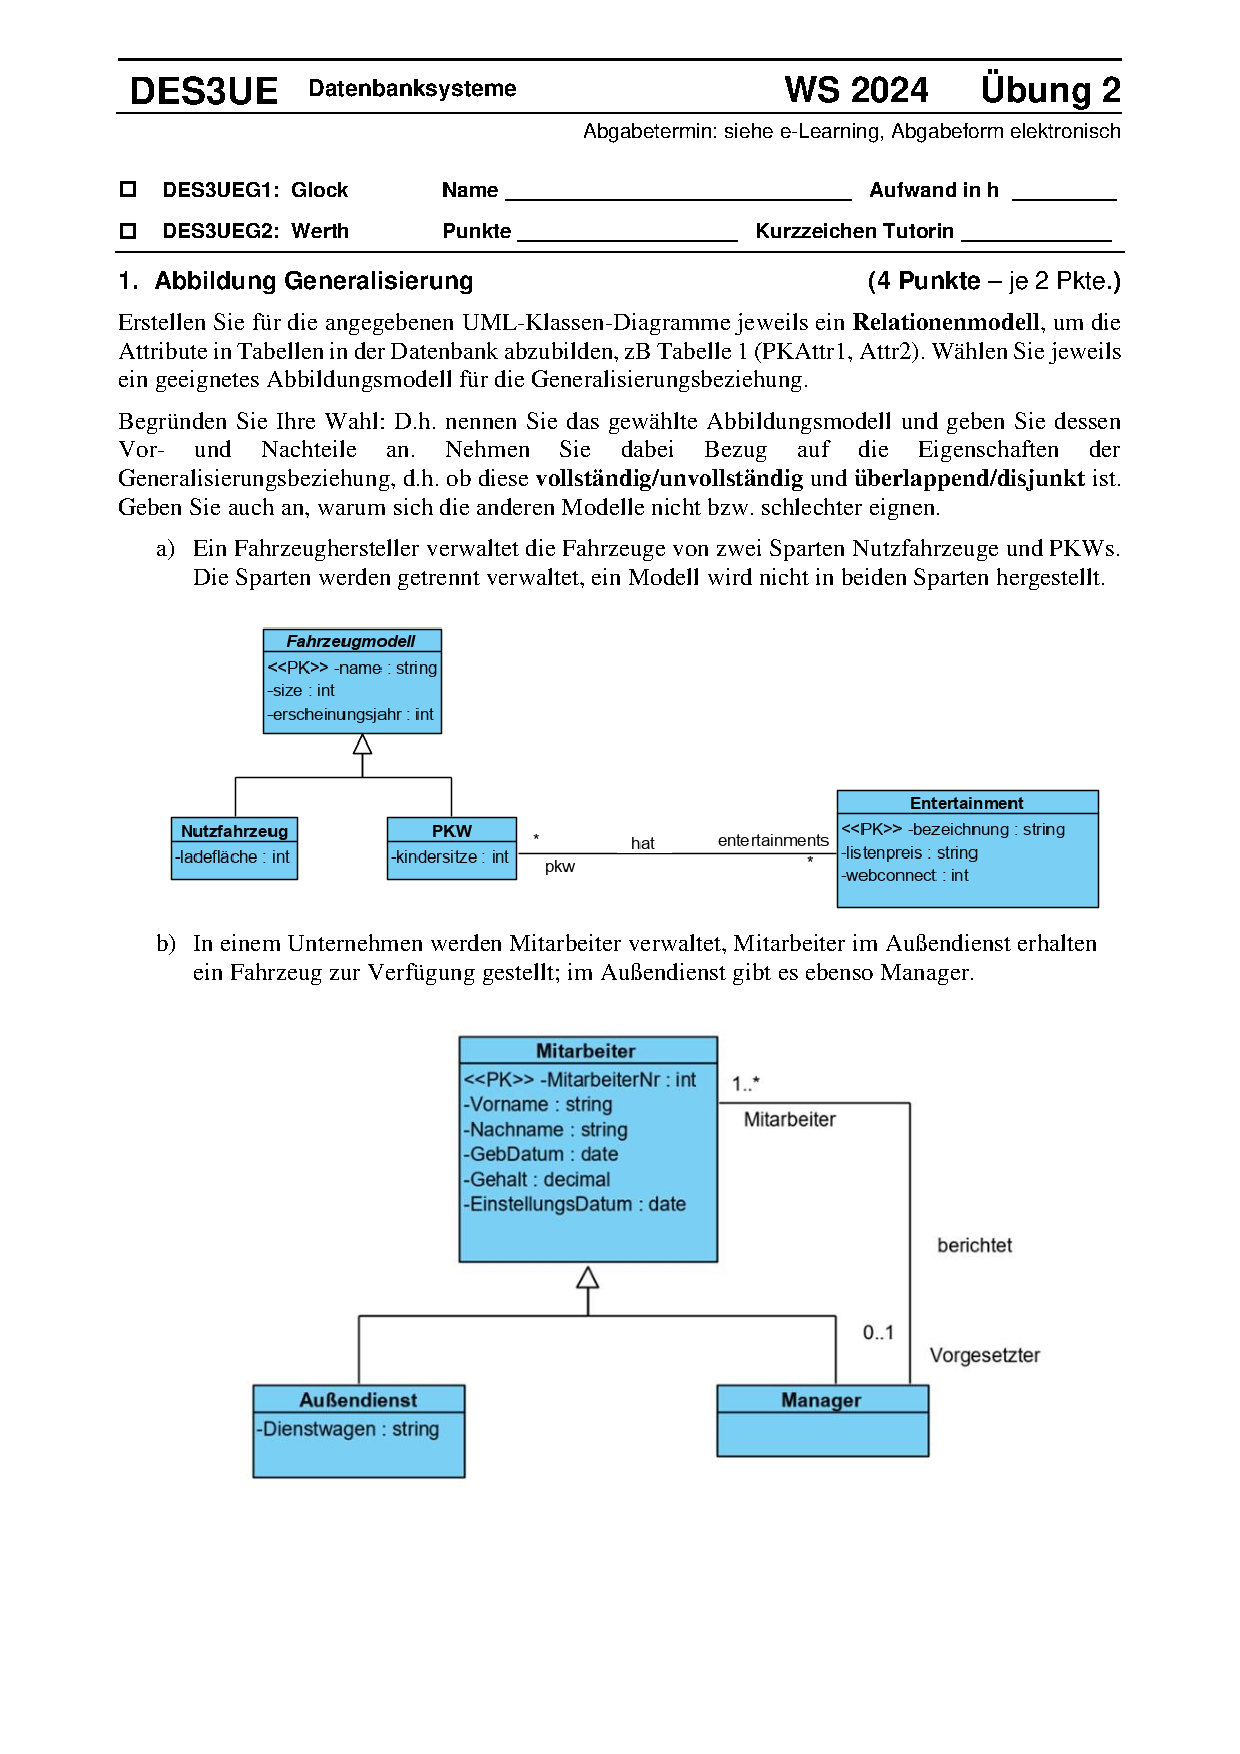
\includegraphics[page=1]{Angabe.pdf}};
	\begin{scope}[shift={(current page.south west)},every node/.style={anchor=base west}]
		\node at (8.5cm, 26.4cm) {\theauthor};
		\node at (17.2cm, 26.4cm) {8};
		\node at (1.87cm, 26.35cm) {X};
	\end{scope}
\end{tikzpicture}

\includepdf[pages=2-4]{Angabe.pdf}

\maketitle
\tableofcontents

\pagebreak

\section{Abbildung Generalisierung}

Die Groß/Kleinschreibung wurde aus der Angabe übernommen.

\subsection{a) Fahrzeuge}

Für die Vollständigkeit der Generalisierung kann man nur Annahmen treffen, da die Angabe nicht ausführlich genug ist.
Ich nehme daher an das die Generalisierung \emph{vollständig} ist.
Aus der Angabe liest man auch heraus das sie \emph{disjunkt} ist.\par

Da es eine \emph{n to m} Beziehung auf eine der Subklassen gibt entscheide ich mich für das Partitionierungsmodell.
Dieses bietet mir die Möglichkeit die Relation nur auf die Subklasse via Foreign Key zu definieren.
Weiters ist sie die einzige Abbilding die die Normalformen einhält.
Performanzweise könnte man über eine Einrelationenabbildung streiten, da man aber die Beziehung nicht richtig abbilden kann fällt diese weg. \par

\subsubsection{Relationenmodell}

\begin{relationalmodel}
	Fahrzeugmodell( &
	\PK{name}, \var{size}, \var{erscheinungsjahr}) \\
	Nutzfahrzeug( &
	\PK{name} : \FK{Fahrzeugmodell}, \var{ladefläche}) \\
	PKW( &
	\PK{name} : \FK{Fahrzeugmodell}, \var{kindersitze}) \\
	Entertainment( &
	\PK{bezeichnung}, \var{listenpreis}, \var{webconnect}) \\
	PKW\_Entertainment( &
	\PK{bezeichnung} : \FK{Entertainment}, \PK{name} : \FK{PKW}) \\
\end{relationalmodel}

\subsection{b) Mitarbeiter}

Dieses Beispiel ist eindeutig \emph{unvollständig} und \emph{überlappend}.\par

Da es wieder eine Beziehung auf eine der Subklassen gibt entscheide ich mich wieder für das Partitionierungsmodell.
Die Einrelationenabbildung wäre wieder möglich und ist, da ein Manager keine Attribute hat, auch sinnvoll, aber man kann nicht über das Model garantieren, dass nur Manager Vorgesetzte sein können.\par

\subsubsection{Relationenmodell}

\begin{relationalmodel}
	Mitarbeiter( &
	\PK{MitarbeiterNr}, \var{Vorname}, \var{Nachname}, \\
	& \var{GebDatum}, \var{Gehalt}, \var{EinstellungsDatum} \\
	& \var{Vorgesetzter} : \FK{Manager}) \\ \\
	Manager( &
	\PK{MitarbeiterNr} : \FK{Mitarbeiter}) \\
	Aussendienst( &
	\PK{MitarbeiterNr} : \FK{Mitarbeiter}, \var{Dienstwagen}) \\
\end{relationalmodel}
\pagebreak

\section{SQL-Wiederholdung}
\inputminted{sql}{../ue2_2.sql}
\pagebreak

\section{Sakila-Statistik}
\inputminted{sql}{../ue2_3.sql}
\pagebreak

\section{Aggregate und Gruppierungen}
\inputminted{sql}{../ue2_4.sql}
\pagebreak

\section{GROUP BY mit GROUPING SETS / ROLLUP}
\inputminted{sql}{../ue2_5.sql}

\subsection{Vergleich der Query Pläne}

\begin{figure}[h]
	\centering
	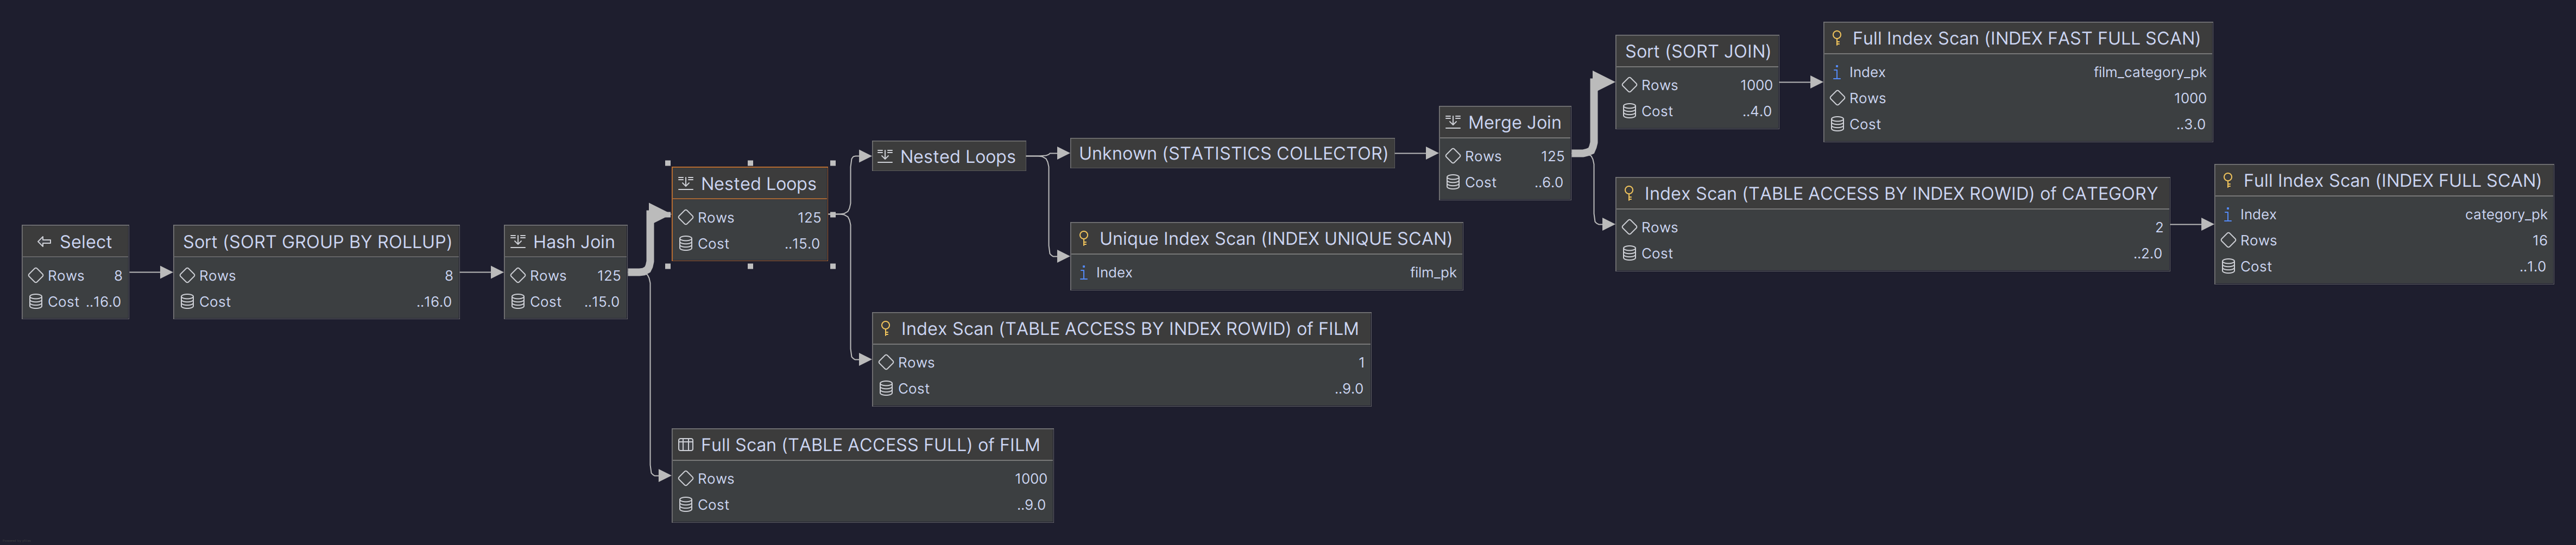
\includegraphics[width=1\linewidth]{../ue2_5_1.png}
	\caption{Queryplan ROLLUP}
\end{figure}
\begin{figure}[h]
	\centering
	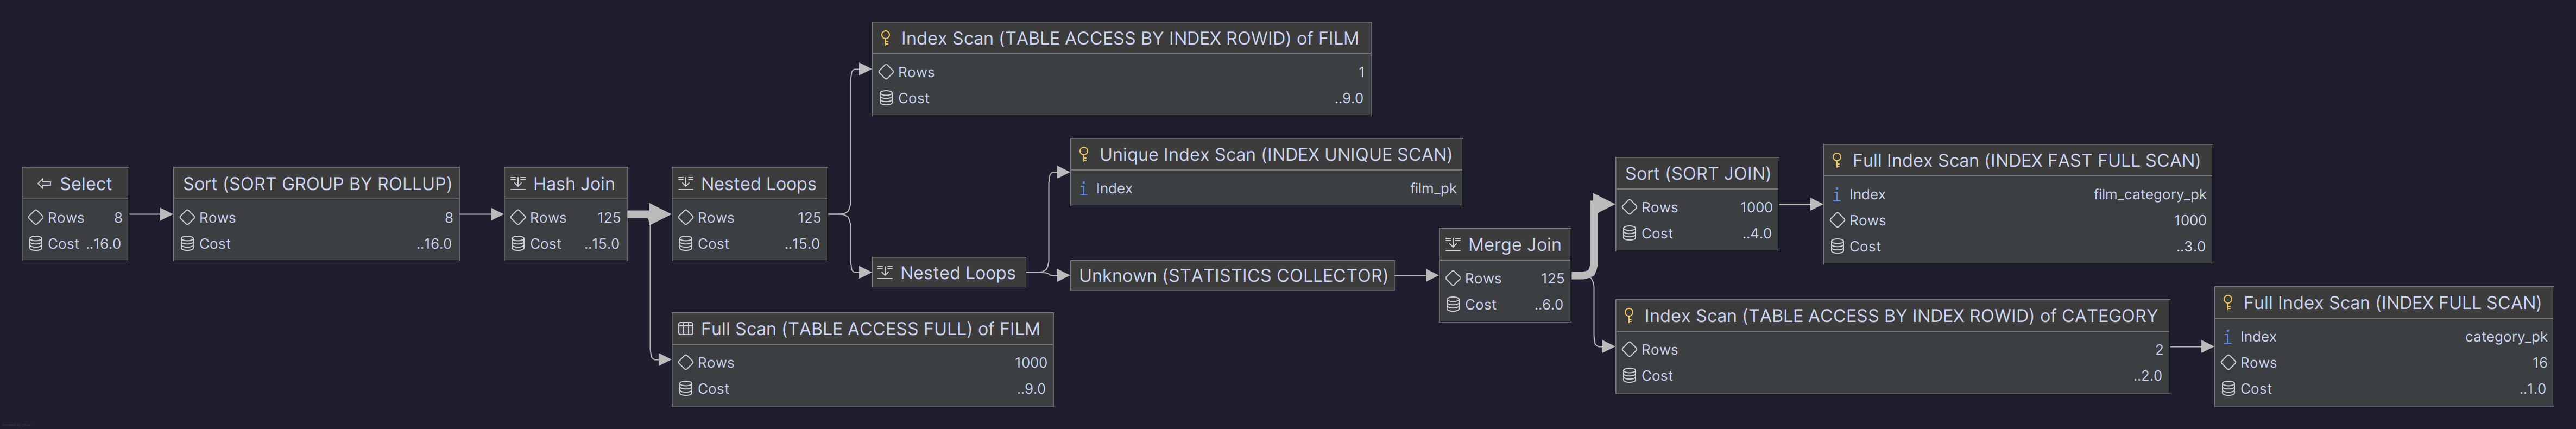
\includegraphics[width=1\linewidth]{../ue2_5_2.png}
	\caption{Queryplan GROUPING SETS}
\end{figure}
\begin{figure}[h]
	\centering
	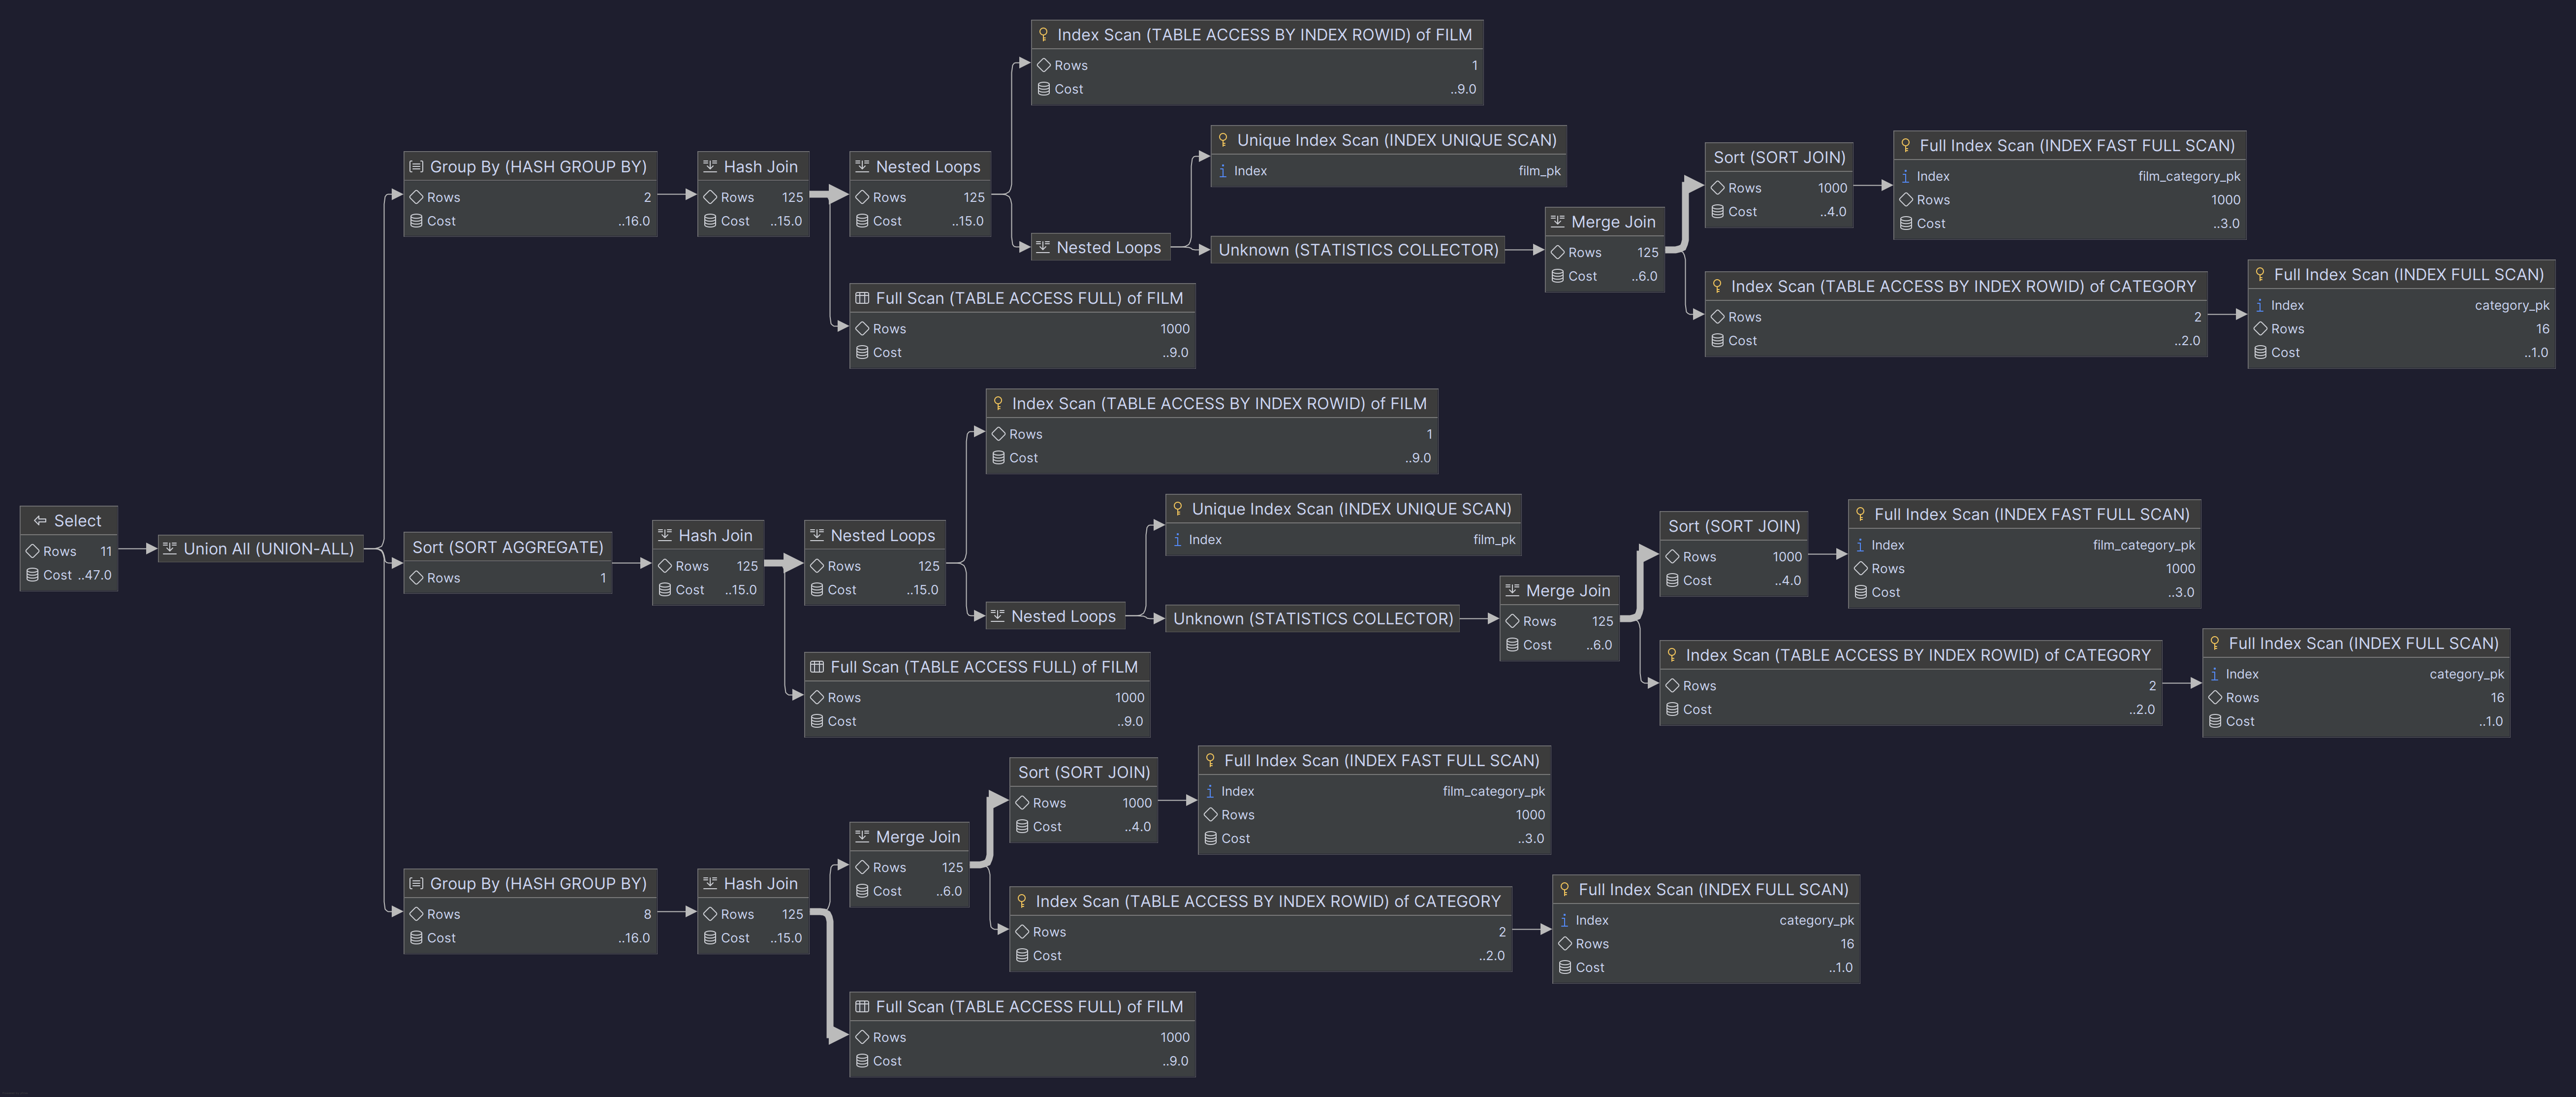
\includegraphics[width=1\linewidth]{../ue2_5_3.png}
	\caption{Queryplan manuelles GROUP BY}
\end{figure}

Wie man sieht optimiert die Datenbank die Querys unterschiedlich.
Die GROUPING SETS und ROLLUP Querys sind sich sehr ähnlich und haben das selbe \emph{weight}.
Die manuelle GROUP BY Query hat ein höheres \emph{weight} und ist daher langsamer, weil durch das UNION mehrfach abgefragt wird.

\section{GROUP BY mit GROUPING SETS / CUBE}
\inputminted{sql}{../ue2_6.sql}
\pagebreak

\end{document}